\chapter{الوراثة والصفات}\label{ch:g9:heredity-and-traits}

صور العائلة معطيات بيولوجية. فذقن الجدة على الطفل
الدارج، وخصلات الأم المجعدة على غير أي من ولديها، وأخ
طويل وأخ ليس كذلك --- الشبه يجري في العائلات، ويجري فيها
الاختلاف كذلك. وقد اتكأ هذا الكتاب على هذه الحقيقة سنين
(مهر \cref{rem:g4:animal-reproduction:mix}، وإخوة
\cref{prop:g8:sexual-reproduction:shuffle})؛ وفصل هذه
السنة الافتتاحي يدرسها أخيرًا: ما الذي يورث بالضبط، وما
الذي لا يورث، وما الذي تتيح لنا أنماط الشبه العائلي أن
نستنتجه.

\begin{omfigure}
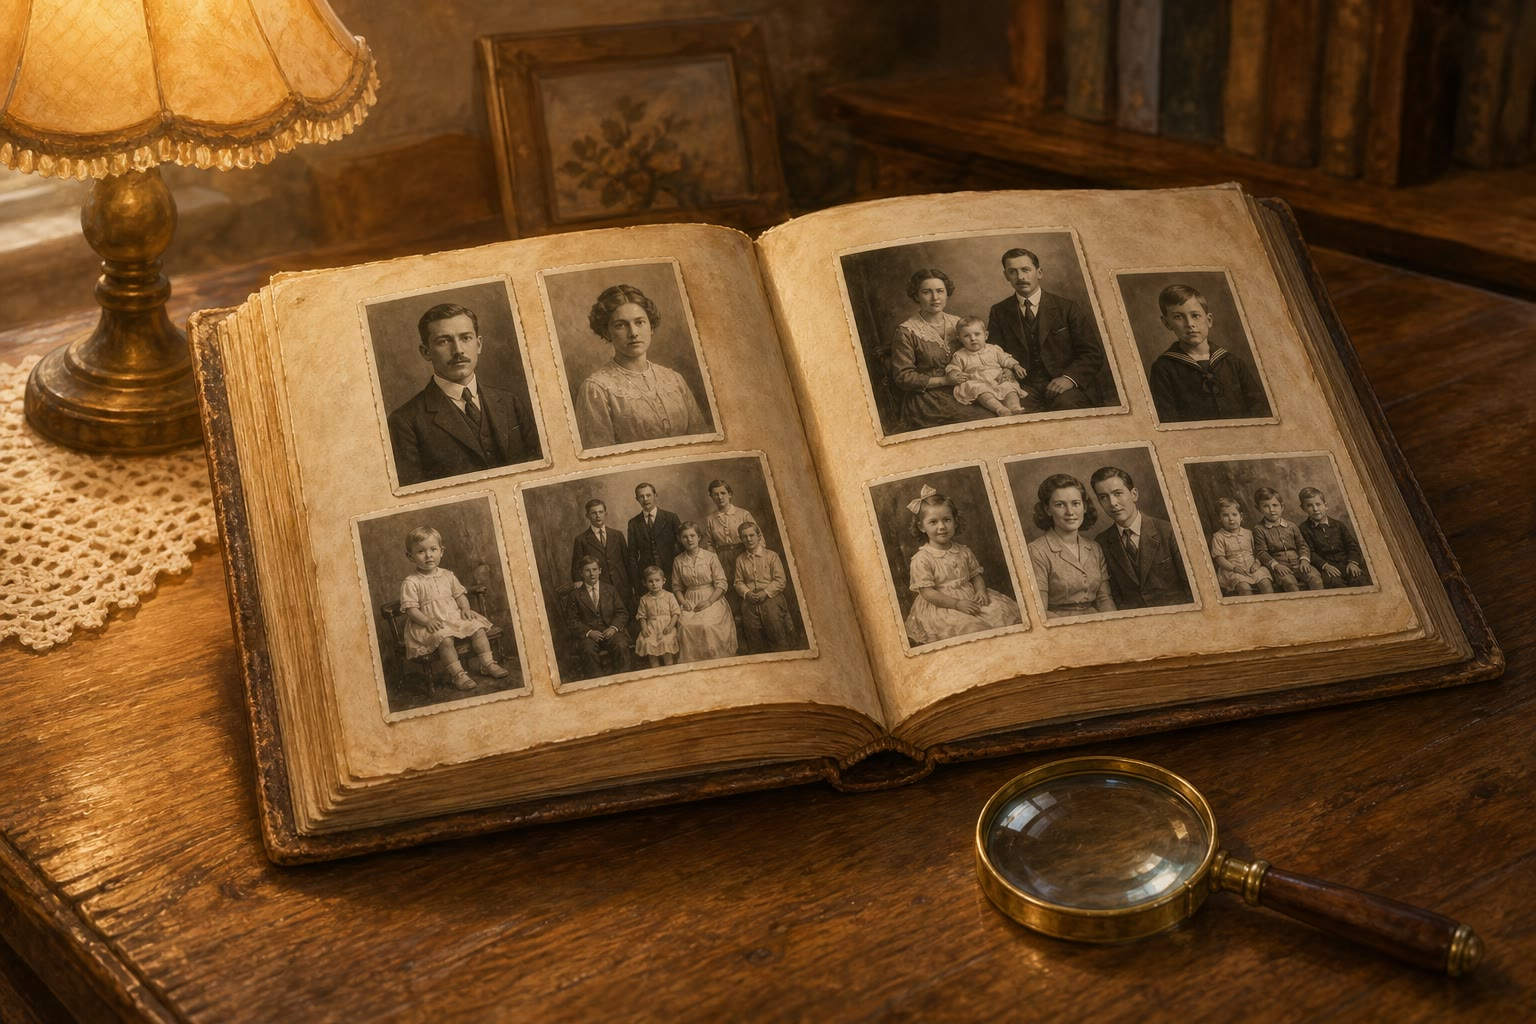
\includegraphics[width=0.62\linewidth]{images/book1/ai/g9-family-album.jpg}

{\small معطيات بيولوجية، بنسخة سمرة الصور القديمة: شبه
واختلاف، يجريان عبر الأجيال.}
\end{omfigure}

\section{الصفات، ومن أين تأتي}

\begin{definition}[الصفات]\label{def:g9:heredity-and-traits:traits}
\emph{الصفة}\index{صفة} كل خاصية يمكن وصفها في فرد ما:
لون \omterm{def:g1:the-five-senses:sense}{العينين}، وزمرة \omterm{prop:g4:journey-of-food:absorb}{الدم}، وشكل شحمة \omterm{def:g1:the-five-senses:sense}{الأذن}، والطول، وصوت
غنائي، وندبة. ومجموع صفات الفرد كلها يبنيه عملان: ما
\emph{ورث}، وما أضافته \emph{\omterm{def:g6:exploring-our-environment:components}{البيئة} والحياة} (عالم
\cref{def:g4:adapted-to-their-world:adaptation}، وهو
يعمل في جسم واحد).
\end{definition}

\begin{definition}[الوراثة]\label{def:g9:heredity-and-traits:heredity}
\emph{الوراثة}\index{وراثة} هي انتقال \omterm{def:g9:heredity-and-traits:traits}{الصفات} من الآباء
إلى الأبناء بالتكاثر --- أي، كما بيّن
\cref{ch:g8:sexual-reproduction}، عبر خليتين مفردتين.
\omterm{def:g9:heredity-and-traits:traits}{والصفات} التي تنتقل بهذا الطريق \emph{وراثية}\index{صفة
وراثية}: فلون \omterm{def:g1:the-five-senses:sense}{العينين} وزمرة \omterm{prop:g4:journey-of-food:absorb}{الدم} وراثيان؛ أما الندوب
وثقوب \omterm{def:g1:the-five-senses:sense}{الأذنين} فليست كذلك، مهما طال حملها. \omterm{def:g3:sorting-living-things:criterion}{ومحك} الفرز هو
\omterm{def:g8:sexual-reproduction:gametes}{الأمشاج}: فما لا تستطيع خليتان حمله لا تستطيع العائلات
نقله.
\end{definition}

\begin{example}[فرز ألبوم عائلي]\label{ex:g9:heredity-and-traits:album}
صور الجد: أنفه المميز --- وراثي، ها هو ذا من جديد عند
العمة وابن العم؛ وسمرة المزارع التي صنعتها الشمس ---
مكتسبة، وحفيده الموظف يفتقر إليها؛ وطوله --- من العملين
جزئيًا، فالحفيد يعلوه على الهيكل نفسه، وقد غذته سنون
أغنى (\cref{prop:g3:balanced-diet:jobs})؛ ومهارته في
الكمان --- غير \omterm{def:g9:heredity-and-traits:heredity}{وراثية} بوصفها مهارة
(\cref{ex:g8:nervous-communication:juggler}: \omterm{def:g8:nervous-communication:synapse}{فالمشابك}
تدرَّب ولا تنقل)، وإن كانت العائلة الموسيقية تخبرنا أن
شيئًا أدق يعمل فيما ينقل: استعدادًا ربما، لا التوصيل
المدرَّب نفسه أبدًا.
\end{example}

\begin{proposition}[الموروث والمكتسب]\label{prop:g9:heredity-and-traits:sorting}
يفترق العملان على ثلاثة \omterm{def:g3:sorting-living-things:criterion}{محكات}:
\begin{enumerate}
  \item \emph{النمط العائلي}: \omterm{def:g9:heredity-and-traits:traits}{الصفات} \omterm{def:g9:heredity-and-traits:heredity}{الوراثية} تتكرر عبر
        الشجرة على خطوط التكاثر؛ أما المكتسبة فتتبع
        الأعمار (فالبحارة كلهم ملوحون، أيًا كان آباؤهم)؛
  \item \emph{الحضور منذ البداية}: زمرة \omterm{prop:g4:journey-of-food:absorb}{الدم} تثبت عند
        \omterm{def:g5:flower-to-fruit:steps}{الإخصاب}؛ أما السمرة والمهارة فتبنيان بعد ذلك؛
  \item \emph{الانتقال}: أبناء مبتوري \omterm{def:g1:my-body:parts}{الأطراف} لهم
        أطرافهم؛ وأبناء لاعبي كمال الأجسام يبدؤون بلا
        تدريب. \omterm{def:g9:heredity-and-traits:traits}{فالصفات} المكتسبة تموت مع مكتسبها ---
        \omterm{def:g8:sexual-reproduction:gametes}{والأمشاج} لا تحملها.
\end{enumerate}
وأكثر \omterm{def:g9:heredity-and-traits:traits}{الصفات} الظاهرة --- الطول، والبنية، بل المزاج ---
منسوجة من العملين معًا: مدى موروث، وملء تعيشه الحياة.
\end{proposition}
\admitted

\section{قراءة الأنماط العائلية}

\begin{example}[صفات تقفز جيلًا]\label{ex:g9:heredity-and-traits:skip}
بعض الأنماط تحير للوهلة الأولى: أبوان بنيا \omterm{def:g1:the-five-senses:sense}{العينين}
وولدهما أزرقهما؛ \omterm{def:g9:heredity-and-traits:traits}{وصفة} للجدة تغيب عن كل أبنائها ثم تعود
عند حفيد. والقفز شائع، وهو يحمل نتيجة ثقيلة: فالوالد
يستطيع أن \emph{ينقل ما لا يظهره}. فتعليمات \omterm{def:g9:heredity-and-traits:traits}{الصفة} سافرت
مستترة عبر جيل --- إذن الموروث ليس \omterm{def:g9:heredity-and-traits:traits}{الصفة} نفسها، بل شيء
\emph{يحددها}، يمكن حمله من غير أن يرى.
\end{example}

\begin{proposition}[ما تلزمنا الأنماط بأن نستنتجه]\label{prop:g9:heredity-and-traits:conclusions}
ثلاث نتائج، تلزم كل واحدة منها ملاحظة:
\begin{enumerate}
  \item لما كانت \omterm{def:g9:heredity-and-traits:traits}{الصفات} المكتسبة لا تنتقل، وجب أن يكون
        المنتقل \emph{محددات} --- تعليمات لبناء \omterm{def:g9:heredity-and-traits:traits}{الصفات}،
        لا \omterm{def:g9:heredity-and-traits:traits}{الصفات} نفسها؛
  \item ولما كانت \omterm{def:g9:heredity-and-traits:traits}{الصفات} تقفز أجيالًا، أمكن أن
        \emph{تحمل المحددات من غير أن تظهر}: فكل فرد
        يحمل أكثر مما يعرض؛
  \item ولما كان كل ولد يتلقى من والديه معًا بمشيجين
        (\cref{prop:g8:sexual-reproduction:core})، أسهم
        كل والد \emph{بانتقاء} من محدداته ---
        والانتقاءات تختلف من ولد إلى ولد، وإلا لتطابق
        الإخوة (خلط
        \cref{prop:g8:sexual-reproduction:shuffle}، وقد
        تحدد موضعه الآن: إنه خلط \emph{للمحددات}).
\end{enumerate}
\end{proposition}
\admitted

\begin{remark}[السؤال الذي يطرحه هذا]\label{rem:g9:heredity-and-traits:question}
لقد حشرنا الألبوم العائلي في سؤال رائع. ففي مكان ما من
لا شيء \omterm{def:g8:reproductive-systems:male}{النطفة} تقريبًا
(\cref{ex:g8:reproductive-systems:sperm} --- \omterm{def:g6:cell-unit-of-life:parts}{نواة} محشوة
وذيل) تسافر تعليمات لأنف، ولزمرة دم، ولون \omterm{def:g1:the-five-senses:sense}{عينين} ---
تحمل من غير أن تظهر، وتنتقى أنصافًا، ويقرؤها الجسم
النامي. \emph{فأين هي، ومم صنعت؟} وتشريح \omterm{def:g8:reproductive-systems:male}{النطفة} يشير إلى
الجواب سلفًا: فكل ما يرسله الأب يسع في \omterm{def:g6:cell-unit-of-life:parts}{نواة}
(\cref{rem:g5:first-look-at-cells:nucleus} وعد بأن لتلك
البقعة شأنًا). والفصلان التاليان يفتحانها.
\end{remark}

\begin{method}[تدقيق صفة]\label{met:g9:heredity-and-traits:audit}
في أي \omterm{def:g9:heredity-and-traits:traits}{صفة}، أجر \omterm{def:g3:sorting-living-things:criterion}{المحكات} الثلاثة:
\begin{enumerate}
  \item ارسمها على \omterm{def:g6:classification-kinship:tree}{شجرة العائلة}: أتتبع خطوط التكاثر، أم
        الأعمار والعادات؟
  \item وأرّخها: أثابتة منذ البداية، أم مبنية في الطريق؟
  \item وطبّق \omterm{def:g3:sorting-living-things:criterion}{محك} \omterm{def:g8:sexual-reproduction:gametes}{المشيج}: أتستطيع خليتان حملها؟ (الندبة
        لا تستطاع؛ وزمرة \omterm{prop:g4:journey-of-food:absorb}{الدم} تستطاع)؛
  \item والحكم: موروثة، أو مكتسبة، أو --- وهو الأشيع ---
        مدى موروث، عيش فيه.
\end{enumerate}
\end{method}

\section{تمارين}

\begin{exercise}[$\star$]\label{exo:g9:heredity-and-traits:1}
عرّف \omterm{def:g9:heredity-and-traits:traits}{الصفة} \omterm{def:g9:heredity-and-traits:heredity}{والوراثة}، وأعط \omterm{def:g3:sorting-living-things:criterion}{محك} الفرز في عبارة واحدة.
\end{exercise}

\begin{exercise}[$\star$]\label{exo:g9:heredity-and-traits:2}
صنّف: زمرة \omterm{prop:g4:journey-of-food:absorb}{الدم}؛ وثقب \omterm{def:g1:the-five-senses:sense}{الأذن}؛ والنمش؛ وطلاقة الفرنسية؛
وشكل شحمة \omterm{def:g1:the-five-senses:sense}{الأذن}.
\end{exercise}

\begin{exercise}[$\star$]\label{exo:g9:heredity-and-traits:3}
اذكر \omterm{def:g3:sorting-living-things:criterion}{المحكات} الثلاثة في
\cref{prop:g9:heredity-and-traits:sorting}.
\end{exercise}

\begin{exercise}[$\star$]\label{exo:g9:heredity-and-traits:4}
لماذا يبدأ أبناء لاعبي كمال الأجسام بلا تدريب؟ وماذا
يبين ذلك؟
\end{exercise}

\begin{exercise}[$\star$]\label{exo:g9:heredity-and-traits:5}
ماذا تثبت \omterm{def:g9:heredity-and-traits:traits}{الصفة} القافزة أن الوالد يستطيع أن يفعله؟
\end{exercise}

\begin{exercise}[$\star$]\label{exo:g9:heredity-and-traits:6}
لماذا وجب أن يكون الموروث محددات لا \omterm{def:g9:heredity-and-traits:traits}{صفات}؟ جملة واحدة.
\end{exercise}

\begin{exercise}[$\star\star$]\label{exo:g9:heredity-and-traits:7}
جاء الطول أعلى عند الحفيد على الهيكل نفسه. فكّك العملين
في تلك الجملة.
\end{exercise}

\begin{exercise}[$\star\star$]\label{exo:g9:heredity-and-traits:8}
فسّر لماذا يختلف الإخوة، بلغة المحددات --- ولماذا لا
يختلف التوأمان المتطابقان
(\cref{exo:g8:from-egg-to-birth:10}).
\end{exercise}

\begin{exercise}[$\star\star$]\label{exo:g9:heredity-and-traits:9}
طبّق \cref{met:g9:heredity-and-traits:audit} على: (أ)
شيب مبكر متكرر في عائلة؛ (ب) قدرة لاعب كرة قدم على
التحمل.
\end{exercise}

\begin{exercise}[$\star\star$]\label{exo:g9:heredity-and-traits:10}
حالة الكمان: ما الذي قد تنقله العائلة الموسيقية، إن لم
تنقل المهارة المدرَّبة أبدًا؟ فرّق بعناية.
\end{exercise}

\begin{exercise}[$\star\star$]\label{exo:g9:heredity-and-traits:11}
أبوان بنيا \omterm{def:g1:the-five-senses:sense}{العينين}، وولد أزرقهما --- والجار يشك في
العائلة. دافع عن العائلة بمنطق
\cref{ex:g9:heredity-and-traits:skip}.
\end{exercise}

\begin{exercise}[$\star\star\star$]\label{exo:g9:heredity-and-traits:12}
من تشريح \omterm{def:g8:reproductive-systems:male}{النطفة} وحده
(\cref{ex:g8:reproductive-systems:sperm})، احتجّ لموضع
محددات الأب --- وما الحجم الذي يستلزمه ذلك لتعليمات
إنسان كامل.
\end{exercise}

\section{مسألة: نسّابة القرية}

\begin{problem}[{مسألة نهاية الأسبوع --- ثلاثة أجيال،
وسجل صفات واحد}]\label{pb:g9:heredity-and-traits:1}
يحشّي نسّابة قرية شجرات عائلات الأبرشية \omterm{def:g9:heredity-and-traits:traits}{بالصفات}: ``ذقن
الكنيسة'' (ذقن مميز يتكرر منذ قرن)، واستعمال اليد
اليسرى، وسعال \omterm{def:g7:how-animals-breathe:four}{رئة} الخبازين من الطحين، وزمر \omterm{prop:g4:journey-of-food:absorb}{الدم} من سجل
التبرع، ووجوه الرعاة الملوحة.

\medskip\noindent\textbf{الجزء الأول --- فرز
السجل.}
\begin{enumerate}
  \item افرز \omterm{def:g9:heredity-and-traits:traits}{الصفات} الخمس وفق
        \cref{met:g9:heredity-and-traits:audit}، مع
        \omterm{def:g3:sorting-living-things:criterion}{المحك} الفاصل في كل واحدة.
  \item السعال يتبع المخبزة لا العائلة: فالزواج داخلها
        يجلبه، والانتقال بعيدًا يفقده. أي \omterm{def:g3:sorting-living-things:criterion}{محك} هذا، وهو
        يعمل؟
  \item ذقن الكنيسة يقفز الجيل الأوسط في فرعين. استخرج
        النتيجة التي يلزم بها.
  \item زمر \omterm{prop:g4:journey-of-food:absorb}{الدم} تفاجئ السجل أحيانًا: ولد من الزمرة O
        لأبوين من الزمرتين A وB. ماذا لا بد أن يكون كل
        والد قد حمله؟
\end{enumerate}

\medskip\noindent\textbf{الجزء الثاني --- القراءة
بالمحددات.}
\begin{enumerate}[resume]
  \item أعد كتابة قرن الذقن بلغة المحددات: ما الذي سافر
        فعلًا عبر أربعة أجيال، وفي أي مركبات
        (\cref{def:g9:heredity-and-traits:heredity})؟
  \item لماذا يختلف أبناء العمومة حاملو الذقن في كل ما
        عداه؟ حدد موضع الخلط.
  \item لا يجد النسّابة حالة واحدة --- في قرن --- انتقلت
        فيها ندبة أو حرفة أو لغة إلى مولود. اذكر
        التعميم، وسببه على مستوى الآلية.
  \item توأما إحدى العائلات متطابقان في الذقن وفيما
        وراءه. بم يخلص السجل عن بدايتهما
        (\cref{rem:g5:human-reproduction:twins})؟
\end{enumerate}

\medskip\noindent\textbf{الجزء الثالث --- المحاضرة.}
\begin{enumerate}[resume]
  \item يحاضر النسّابة: ``تنقل الأبرشية إرثين --- إرثًا
        \omterm{def:g8:sexual-reproduction:gametes}{بالأمشاج}، وإرثًا بالعيش معًا.'' أسند \omterm{def:g9:heredity-and-traits:traits}{صفات} السجل
        الخمس إلى القناتين.
  \item ``كل واحد منا يعرض أقل مما يحمل.'' دافع عن ذلك
        من السجل، مرتين.
  \item يسأل مستمع ما تعليمات قناة \omterm{def:g8:sexual-reproduction:gametes}{الأمشاج} ماديًا. أعط
        جواب \cref{rem:g9:heredity-and-traits:question}
        الصادق --- الموضع معروف، والمحتوى في الفصل
        التالي.
  \item اختم المحاضرة بحكم التدقيق في سطر عن الحالة
        الأشيع: أكثر \omterm{def:g9:heredity-and-traits:traits}{الصفات} \emph{ماذا}، معيشًا
        \emph{كيف}؟
\end{enumerate}
\end{problem}
